\documentclass{article}
\usepackage[utf8]{inputenc}
\usepackage{amsmath}
\usepackage{setspace}
\usepackage{mathtools}
\usepackage{amssymb}
\usepackage{amsfonts}
\newcommand\der[2]{\frac{\partial{#1}}{\partial{#2}}}
\usepackage{sectsty}
\usepackage[parfill]{parskip}
\usepackage{changepage}   % for the adjustwidth environment
\usepackage{graphicx}
\graphicspath{ {./Pictures/} }
\usepackage{float}
\usepackage[margin=1in]{geometry}
\setlength{\parindent}{0em}
\sectionfont{\fontsize{12}{12}\selectfont}
\nonfrenchspacing
\renewcommand{\baselinestretch}{1.5}
\usepackage{indentfirst}
\usepackage{enumitem}
\setlist[itemize]{topsep=0pt,itemsep=0pt,partopsep=0pt,parsep=0pt}
\usepackage{xcolor}
\usepackage{titlesec}
\DeclareUnicodeCharacter{2212}{-}
\usepackage{tikz}
\usetikzlibrary{calc}
\newcommand{\tikzmark}[1]{\tikz[overlay,remember picture] \node (#1) {};}
\titleformat{\section}[block]{\color{blue}\Large\bfseries\filcenter}{}{1em}{}
\usepackage[normalem]{ulem}
\usepackage{calrsfs}
\renewcommand{\labelitemiv}{$\circledast$}
\renewcommand{\labelitemii}{$\circ$}

\title{Macroeconomics A Notes}
\author{Nicholas Umashev \footnote{content is not of my own authorship}}
\date{2019}

\begin{document}

\maketitle

\tableofcontents

\newpage

\section{Consumer Theory}

\vspace{2.5mm}
\subsection{Mathematical Concepts}
\subsubsection{Consumption/Choice Set X}
The set of all alternative, or complete consumption plans, that the consumer can conceive -whether achievable or note
\begin{itemize}
  \item  \underline{Alternative Definition}: the consumpsion set is the entire non-negative orthan, $X = \mathbb{R}^{n}_{+}$
  \item  \underline{Consumption Bundle}: a consumption bundle of $n$ goods is defined as a vector $x == (x_{1}, \dots, x_{n}) \in \mathbb{R}_{+}^{n}$, specifying the quantities of the $n$ available commodities
  \item  \underline{Properties of Consumption Set}: (1) $X \subseteq \mathbb{R}_{+}^{n}$, (2) $X$ is closed, (3) $X$ is convex, (4) $0 \in X$
\end{itemize}
\subsubsection{Complements of Sets}
For a given subset $A \subseteq X$, we define the complement of $A$ in $X$ to be the set $A^{c} = \left\{ x \in X: x \notin A \right\}$
\begin{itemize}
  \item \underline{Alternative Definition}: the complement set of set $A$ in $X$ is all the stuff in the universe $X$ that is not in $A$
  \item  \underline{Application}: typically we define either \textit{open sets} or \textit{closed sets} and the other (\textit{closed} or \textit{open}) as the complement of the first
\end{itemize}
\subsubsection{Metric Distance}
In huge space $\mathbb{R}_{+}^{n}$, open balls (neighbourhoods) are determined using a metric distance function
\begin{itemize}
  \item  \underline{Euclidean Metric}: measures the distance between two points $x, y \in \mathbb{R}_{+}^{n}$ as $d(x,y) = \sqrt{\sum_{i=1}^{n}(x_{i}-y_{i})^{2}}$
  \begin{itemize}
    \item  \underline{n-Dimensional Spaces}: in a two dimensional space this is equivalent to $d(x,y) == \sqrt{(x_{1} - y_{1})^{2} + (x_{2} = y_{2})^{2}}$, while in a one dimensional space this is equivalent to $d(x,y) = \sqrt{(x_{1} - y_{1})^{2}} = x_{1} - y_{1}$
    \item  \underline{Triangular Inequality}: for all $x, y, z \in \mathbb{R}_{+}^{n}$, $d(x,y) \leq d(x,z) + d(z,y)$
  \end{itemize}
  \item  \underline{Euclidean Metric Example}: the distance between $x = (2,2)$ and $y = (1,4)$ is $d(x,y) = \sqrt{(2-1)^{2} + (2-4)^{2}} = \sqrt{5}$
  \begin{itemize}
    \item  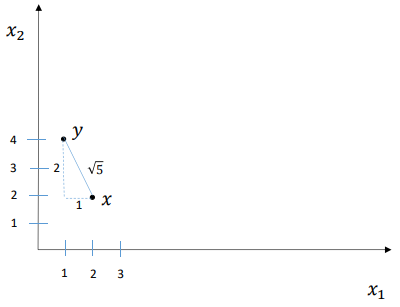
\includegraphics[width=5cm, height=3cm]{pic1}
  \end{itemize}
\end{itemize}
\subsubsection{Open Balls (neighborhoods)}
An open ball $B_{\varepsilon}(x) = \left\{ y \in \mathbb{R}_{+}^{n}: d(x,y) < \varepsilon \right\}$ is the set of points that are closer in Euclidean distance to $x \in \mathbb{R}_{+}^{n}$ than some real number $\varepsilon > 0$
\begin{itemize}
  \item  \underline{Alternative Definition}: the open ball $B_{\varepsilon}(x)$ with radius $\varepsilon > 0$ and center $x \in \mathbb{R}^{m}$ is the set of points $y \in \mathbb{R}^{m}$ with distance less than $r$ from $x$, i.e. $B_{\varepsilon}(x) = \left\{ y \in \mathbb{R}^{m}: \ ||y - x|| < \varepsilon \right\}$
  \begin{itemize}
    \item  \underline{Note}: the theorem must contain $<$ instead of $\leq$ because otherwise the ball would contain its boundary points making it a closed instead of open ball. In otherwords, for an open ball each point in the element must be less than a selected radius on a plane
  \end{itemize}
  \item  \underline{Example 1}: in $\mathbb{R}_{+}^{1}$ an open ball is an open interval on the number line. For $B_{1.5}(3)$ the circles at the endpoints of the interval $(1.5, 3.5)$ indicate that $1.5$ and $3.5$ are not in the open ball
  \begin{itemize}
    \item  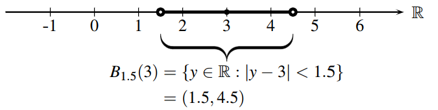
\includegraphics[width=5cm, height=3cm]{pic2}
  \end{itemize}
  \item  \underline{Example 1}: for $x = (2,2)$ and $\varepsilon = 1$, the open ball $B_{\varepsilon}((2,2)) = \left\{ y \in \mathbb{R}^{n}_{+}: \ \sqrt{(y_{1} - 2)^{2} + (y_{2} - 2)^{2}} < 1 \right\}$
  \begin{itemize}
    \item  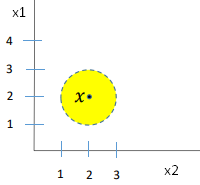
\includegraphics[width=5cm, height=3cm]{pic3}
  \end{itemize}
\end{itemize}
\subsubsection{Open Set}
A set $A \subseteq \mathbb{R}_{+}^{n}$ is open if and only if for each point $x \in A$ there is a radius $\varepsilon_{x} > 0$ such that the open ball $B_{\varepsilon}(x) \subseteq A$
\begin{itemize}
  \item  \underline{Alternative Definition}: a set $S \in \mathbb{R}^{m}$ is open if and only if for each $x \in S$ there exists an open ball around $x$ that is completely contained in $S$
  \item  \underline{Boundary Points}: open sets cannot contain their boundary points, in other words the limit is not in the set since there is no open ball around $limit_{x}$ that is entirely in S. This distinguishes open sets from closed sets
  \item  \underline{Theorem 1}: every open ball $A = B_{\varepsilon}(x)$ is an open set
  \begin{itemize}
    \item  \underline{Proof Outline}: take an arbitrary point $y$ in $B_{\varepsilon}(x)$ and prove that any arbitrary point $z$ contained in $B_{\varepsilon'}(y)$ is also contained in $B_{\varepsilon}(x)$
    \item  \underline{Proof}: take an arbitrary point $y$ in $B_{\varepsilon}(x)$. We need to show that there is an open ball $B_{\varepsilon'}(y)$ around $y$ that is contained in $B_{\varepsilon}(x)$. To do this, we prove that taking an arbitrary point $y$ in $B_{\varepsilon}(x)$ implies that $d(x,y) < \varepsilon$. Since $\varepsilon' = \varepsilon - d(x,y) > 0$, we have that $d(x,y) = \varepsilon - \varepsilon'$. Using $d(x,y) = \varepsilon - \varepsilon'$ and picking an arbitrary $z \in B_{\varepsilon'}(y)$ we can show that $d(x,z) < \varepsilon$. By triangular inequality, $d(x,z) \leq d(x,y) + d(y,z)$ and plugging $d(x,y) = \varepsilon - \varepsilon'$ into this yields $d(x,z) \leq \varepsilon - \varepsilon' + d(y,z)$. Since $z$ is contained in $B_{\varepsilon'}(y)$, it must be that $d(y,z) < \varepsilon'$. Using $d(y,z) < \varepsilon'$ yields $d(x,z) \leq \varepsilon - \varepsilon' + d(y,z) < \varepsilon$ (since $d(y,z)$ is counteracted by $\varepsilon'$ it cannot be the cause of the RHS being greater than the LHS) and therefore $d(x,z) < \varepsilon$. Since every point $z$ is contained in $B_{\varepsilon'}(y)$, $d(x,z) < \varepsilon$ implies that $d(x,y) < \varepsilon$. Therefore, $B_{\varepsilon'}(y) \subseteq B_{\varepsilon}(x)$.
    \item  \underline{Logic}: since $\varepsilon$ can be infinitismal, the infinitismal open ball $B_{\varepsilon}(y)$ contained in the open ball $B_{\varepsilon}(x)$ does not contain the boundary points of $B_{\varepsilon}(x)$
  \end{itemize}
  \item  \underline{Theorem 2}: $A = \mathbb{R}^{n}$ is open in $\mathbb{R}^{n}$, $A = \mathbb{R}^{n}_{+}$ is open in $\mathbb{R}^{n}_{+}$
  \begin{itemize}
    \item  \underline{Logic 1}: take a point on the boundary. Since, by definition, open balls only include elements contained in $\mathbb{R}^{n}$ then any open ball that goes around the boundary point excludes points outside $\mathbb{R}^{n}$. The same is true for $R^{n}_{+}$ if we consider only positive natural numbers in our universe and therefore restrict the definition of open balls to only include points in $\mathbb{R}_{+}^{n}$. In otherwords, every point that is in the ball is in the universe
    \item  \underline{Logic 2}: take any point $x \in A$ and let $\varepsilon_{x} = \min \left\{x_{1}, x_{2}, \dots, x_{n} \right\}$. Then every point in the open ball $B_{varepsilon_{x}}(x) \in \mathbb{R}_{+}^{n}$. For example, let $x = (3,4) \in R_{+}^{2}$ and therefore $\varepsilon_{x} = \min \left\{ 3, 4 \right\} = 3$ - every point $y$ in the open yellow ball will be in $\mathbb{R}_{+}^{2}$ since each point $y$ satisfies $y_{i} > 0$ for $i = 1, 2$.
  \end{itemize}
  \item  \underline{Theorem 3}: $A = \varnothing$ is open in $\mathbb{R}_{+}^{n}$
  \begin{itemize}
    \item  \underline{Proof}: observe that the conditions of openness of a set is satisfied if each $x \in A$ has an open neighbourhood in $A$. Since there is no $x$ in $A = \varnothing$, it follows that each $x \in A$ has an open ball in $A$
    \item  \underline{Both Open and Closed}: the empty set $\varnothing$ is both open and closed, this is as $\forall x \in \varnothing$ $x$ is an interior point (i.e. is open) and since the set of boundary points of $\varnothing$ is the empty set (i.e. is closed)
    \begin{itemize}
      \item  \underline{Complement}: since the complement of $A = \varnothing$ is $\mathbb{R}_{+}^{n}$ and the complement of $A = \mathbb{R}_{+}^{n}$ is $\varnothing$ then both $\mathbb{R}_{+}^{n}$ and $\varnothing$ are closed
    \end{itemize}
  \end{itemize}
\end{itemize}
\subsubsection{Closed Set}
A set $A \subset \mathbb{R}_{+}^{n}$ is closed if and only if the complement $A^{c} = \left\{ x \in \mathbb{R}_{+}^{n}: \ x \notin A \right\}$ of A is an open set
\begin{itemize}
  \item  \underline{Alternative Definition}: a set $S \in \mathbb{R}^{m}$ is closed if, whenever $\left\{ x_{n} \right\}_{n=1}^{\infty}$ is a convergent sequence completely contained in $S$, its limit is also contained in $S$ - in other words, a set $S \subseteq \mathbb{R}^{m}$ is closed if it contains all of its boundary points
  \item  \underline{Example 1}: continuing from example 1 of open balls, the complement of the yellow open ball is a closed set. Formally, this is the entire positive quadrant excluding the yellow open ball, $A^{c} = \left\{ x \in \mathbb{R}_{+}^{n}: \ x \notin B_{1}((2,2)) \right\}$
  \begin{itemize}
    \item  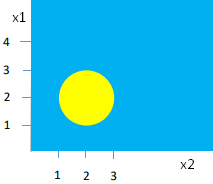
\includegraphics[width=5cm, height=3cm]{pic4}
  \end{itemize}
\end{itemize}
\subsubsection{DeMoran's Laws}
(Law 1) the complement of the union of any family of sets is equal to the intersection of the complements of the family \\ (Law 2) the complement of the intersection of any family of sets is equal to the union of the complements of the family
\begin{itemize}
  \item  \underline{Implications}: (1) the empty set $\varnothing$ and universal set $\mathbb{R}_{+}^{n}$ are both closed and open, (2) the union of any finite family of closed(open) sets is closed(open), (3) the intersection of any family of closed(open) sets is closed(open)
  \begin{itemize}
    \item  \underline{Finite Intersection Logic}: if we take the intersection of two finite open sets $A = \cap_{K \in \mathbb{N}} (1 - \tfrac{1}{k}, 1 + \tfrac{1}{k})$ then only $1 \in A$ and $A = \left\{ 1 \right\}$ is not open
    \item  \underline{Note}: implications 2 and 3 arise by combining Law 1 and Law 2
  \end{itemize}
\end{itemize}
\subsubsection{Bounded Set}
A set $A \subseteq \mathbb{R}_{+}^{n}$ is bounded if and only if we can put an open ball in $\mathbb{R}^{n}$ around the set $A$
\begin{itemize}
  \item  \underline{Alternative Definition}: a set is bounded if there is an open ball that contains it, i.e. $S \subseteq R^{m}$ is bounded if $\exists K > 0: \ ||x|| < K, \ \forall x \in S $
  \item  \underline{Example}: the left image is bounded, the right is not bounded
  \begin{itemize}
    \item  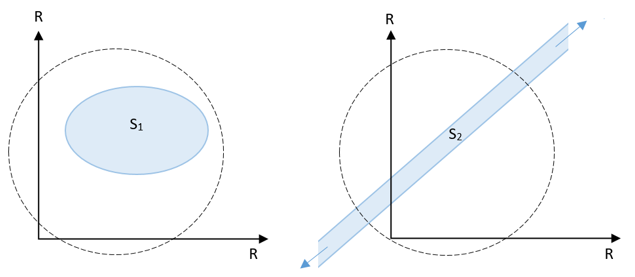
\includegraphics[width=5cm, height=3cm]{pic5}
  \end{itemize}
\end{itemize}
\underline{Compact Set}: a set $A \subseteq \mathbb{R}_{+}^{n}$ is bounded if and only if it is both closed and bounded
\begin{itemize}
  \item  \underline{Example}: $B_{1} = \left\{ (x_{1},x_{2}) \in mathbb{R}^{2}: p_{1}x_{1} + p_{2}x_{2} \leq w \right\}$ is closed but not bounded. However, $B_{2} = \left\{ (x_{1},x_{2}) \in \mathbb{R}^{2}: p_{1}x_{1} + p_{2}x_{2} \leq w, x_{1} \geq 0, x_{2} \geq 0 \right\}$ is closed and bounded and therefore compact.
\end{itemize}
\subsubsection{Convex Set}
A set $A \subseteq \mathbb{R}_{+}^{n}$ is a convex set if and only if for all $x, y \in A$, and each $\alpha \in [0,1]$, the point $\alpha x + (1- \alpha)y$ is also in A
\begin{itemize}
  \item  \underline{Alternative Definition}: a set $S \subseteq \mathbb{R}^{n}$ is convex if and only if for every two points of the set the line segment between the two points also belongs to the set
  \item  \underline{Example}: parts (a) and (b) are convex sets since all points between any two points are contained in the set, parts (c) and (d) are not convex sets since they contain two points where points between them are not contained in the set
  \begin{itemize}
    \item  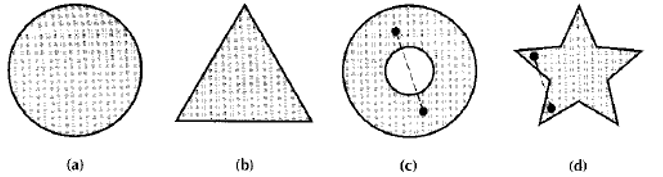
\includegraphics[width=5cm, height=3cm]{pic8}
  \end{itemize}
\end{itemize}
\subsubsection{Convergence}
For all $\varepsilon > 0$ there exists a $\mathbb{N}$ such that for all values of $n$ greater than $\mathbb{N}$ the $n^{th}$ \textit{elements value in the sequence minus the limit's value} will be less than $\varepsilon$
\begin{itemize}
  \item  \underline{Mathemtical Definition}: let $(x_{n})_{n \in \mathbb{N}}$ be a sequence with codomain $\mathbb{R}$. We say that $(x_{n})$ converges to $x^{*}$ or that $x^{*}$ is the limit of $(x_{n})_{n \in \mathbb{N}}$ if: $\forall \varepsilon > 0 \exists N \in \mathbb{N} \forall n \geq N: \ |x_{n} - x^{*}| < \varepsilon$
\end{itemize}
\subsubsection{Continuous Function}
A function $f: \mathbb{R}_{+}^{n} \rightarrow \mathbb{R}$ is continuous if and only if the inverse image $f^{-1} (B) = \left\{ x \in \mathbb{R}_{+}^{n}: f(x) \in B \right\}$ of each open ball $B$ in the range $\mathbb{R}$ is also open in the doman $\mathbb{R}_{+}^{n}$
\begin{itemize}
  \item  \underline{Alternative Definition 1}: a function that maps nearby points into nearby points - i.e. you can draw the graph of the function without lifting your pencil from the paper. In other words, if we want to get all the $f(x)$ values to stay in some small neighborhood around $f(x_{0})$ we simply need to choose a small enough neighborhood for the $x$ values around $x_{0}$. If we can do that no matter how small the $f(x)$ neighborhood is, then $f$ is continuous at $x_{0}$
  \item  \underline{Alternative Definition 2}: let $D \subseteq \mathbb{R}^{k}$. A function $f: D \rightarrow \mathbb{R}^{m}$ is continuous at $x = (x_{1}, x_{2}, \dots, x_{k}) \in D$ if for every sequence $(x_{n})_{n \in \mathbb{N}} \in D$ that converges to x, the sequence $(f(x_{n}))_{n\in \mathbb{N}} \in \mathbb{R}$ converges to $f(x)$. The function is continuous if it is continuous at $x$ for all $x \in D$
  \item  \underline{Alternative Definition 3}: continuity of $f: D \rightarrow R$ at $x_{0} \in D$ means that for every $\varepsilon > 0$ there exists a $\delta > 0$ such that for all $x \in D$: $$|x - x_{0}| < \delta \Rightarrow |f(x) - f(x_{0})| < \varepsilon $$
  \item  \underline{Continuous Example}: the below function is continuous as for any $x_{0}$ that we select and converges, the codomain converges to $y_{0}$
  \begin{itemize}
    \item  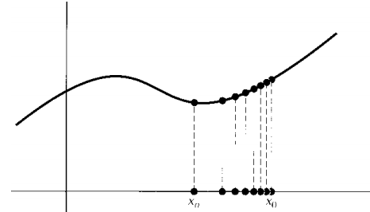
\includegraphics[width=5cm, height=3cm]{pic6}
  \end{itemize}
  \item  \underline{Discontinuous Example}: the function $f(x) = \left\{ 1 \ \text{if} \ x > 0, 0 \ \text{if} \ x \leq 0 \right\}$ is not continuous as the codomain does not converge to the $y_{0}$ given by the $x_{0}$ selected. In other words, for $\varepsilon < 1$ the definition of convergence is violated at $x_{0} = 0$
  \begin{itemize}
    \item  
\includegraphics[width=5cm, height=3cm]{pic7}
  \end{itemize}
  \item  \underline{Using original definition}: the image of $f(x)$ consists of all the elements of $y$ that an element of $x$ is mapped to. If $f(x) = \left\{x \ \text{if} \ x < 10, x + 10 \ \text{if} \ x \geq 10 \right\}$ and we set the inverse image open ball $B = (15, 25)$, then  we have that $f^{-1}(15,25) = \left\{ x \in \mathbb{R}: \ f(x) \in (15, 25) \right\} = [10, 15)$. \begingroup\color{magenta} The set $[10, 15)$ is not open in the domain \endgroup
\end{itemize}

\vspace{2.5mm}
\subsection{Preferences}
\subsubsection{Preference Relation}
Preferences are defined for each consumer over bundles of goods, with the notation $\succeq$ meaning "at least as good as"
\begin{itemize}
  \item \underline{Preferences Definition}: preferences of a consumer on the set of bundles in $\mathbb{R}_{+}^{n}$ (i.e. a single bundle) is a subset $\succeq$ of $\mathbb{R}_{+}^{n} \times \mathbb{R}_{+}^{n}$ (i.e. all possible bundles available). In mathematics, this subset is referred to as a \textit{binary relation} on the set $\mathbb{R}_{+}^{n}$
  \begin{itemize}
    \item  \underline{Note}: there are many preferences that are allowed as there are many subsets of $\mathbb{R}_{+}^{n} \times \mathbb{R}_{+}^{n}$
  \end{itemize}
  \item  \underline{Examples}
  \begin{itemize}
    \item  \underline{Example 1}: $\succeq = \mathbb{R}_{+}^{n} \times \mathbb{R}_{+}^{n}$ represents the case where every possible bundle is at least as good as every other
    \item  \underline{Example 2}: $\succeq = \varnothing$ represents the case where no bundle is at least as good as any other (including itself
    \item  \underline{Example 3}: $\succeq = \left\{ (x,y) \in \mathbb{R}_{+}^{n} \times \mathbb{R}_{+}^{n}: \ x_{i} \geq y_{i} \ \text{for all} \ i = 1, \dots, n \right\}$ represents the case where only bundles where one has at least as much of each good as the other can be compared
    \item  \underline{Example 4}: $\succeq = \left\{ (x,y) \in \mathbb{R}_{+}^{n} \times \mathbb{R}_{+}^{n}: \ \prod_{i=1}^{n} x_{i} \geq \prod_{i=1}^{n} y_{i} \right\}$ represents the case where all bundles are compared and on is at least as good as another whenever the product of quantities is higher. See below for a graphical representation where $x_{1}x_{2} = 2$, red represents the better than sets and blue the worse than sets
    \begin{itemize}
      \item  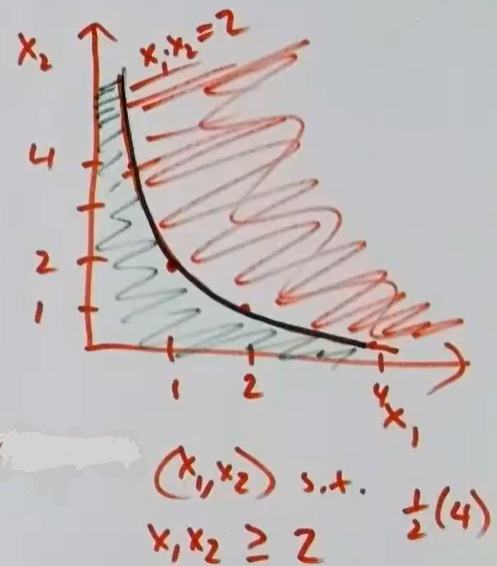
\includegraphics[width=4cm, height=3cm]{pic12}
    \end{itemize}
  \end{itemize}
\end{itemize}
\subsubsection{Strict and Indifferent Preference Relations}
  \begin{itemize}
    \item  \underline{Strict Preference Relation}: when the binary relation $\succ$ on the consumption set $X$ is defined as follows; $x_{1} \succ x_{2}$ if and only if $x_{2} \nsucceq x_{1}$. This is read $x_{1}$ is strictly preferred to $x_{2}$
    \begin{itemize}
      \item  \underline{Implication 1}: from $\succeq = \mathbb{R}_{+}^{n} \times \mathbb{R}_{+}^{n}$ we have that $\succ = \varnothing$ and therefore there is no strict preference
      \item  \underline{Implication 2}: from $\succeq = \varnothing$ we have that $\succeq = \varnothing$ and therefore none are strict
      \item  \underline{Implication 3}: from $\succeq = \left\{ (x,y) \in \mathbb{R}_{+}^{n} \times \mathbb{R}_{+}^{n}: \ x_{i} \geq y_{i} \ \text{for all} \ i = 1, \dots, n \right\}$ we get that $$\succ = \left\{ (x,y) \in \mathbb{R}_{+}^{n} \times \mathbb{R}_{+}^{n}: \ x_{i} \geq y_{i} \ \text{for all} \ i = 1, \dots, n \ \text{and} \ x_{i}>y_{j} \ \text{for some} \ j = 1, \dots, n \right\}$$Therefore, a bundle is strictly preferred to $y$ if and only if $x$ has  at least as much of each commodity as y and stricty more of some commodity
      \item  \underline{Implication 4}: from $\succeq = \left\{ (x,y) \in \mathbb{R}_{+}^{n} \times \mathbb{R}_{+}^{n}: \ \prod_{i=1}^{n} x_{i} \geq \prod_{i=1}^{n} y_{i} \right\}$ we get that $$\succ = \left\{ (x,y) \in \mathbb{R}_{+}^{n} \times \mathbb{R}_{+}^{n}: \ \prod_{i=1}^{n} x_{i} > \prod_{i=1}^{n} y_{i} \right\}$$Therefore, we have strict preference only when the product is higher
    \end{itemize}
    \item  \underline{Indifference Relation}: when the binary relation $\sim$ on the consumption set $X$ is defined as follows; $x_{1} \sim x_{2}$ if and only if $x_{1} \succeq x_{2}$ a nd $x_{2} \succeq x_{1}$. This is read as $x_{1}$ is indifference to $x_{2}$
    \begin{itemize}
      \item  \underline{Implication 1}: from $\succeq = \mathbb{R}_{+}^{n} \times \mathbb{R}_{+}^{n}$ we have that $\sim = \mathbb{R}_{+}^{n} \times \mathbb{R}_{+}^{n}$ and therefore all bundles are indifferent
      \item  \underline{Implication 2}: from $\succeq = \varnothing$ we get $\sim = \varnothing$
      \item  \underline{Implication 3}: from $\succeq = \left\{ (x,y) \in \mathbb{R}_{+}^{n} \times \mathbb{R}_{+}^{n}: \ x_{i} \geq y_{i} \ \text{for all} \ i = 1, \dots, n \right\}$ we get that $$\sim= \left\{ (x,y) \in \mathbb{R}_{+}^{n} \times \mathbb{R}_{+}^{n}: \ x = y \right\}$$Therefore, each bundle is indifferent only to itself
      \item  \underline{Implication 4}: from $\succeq = \left\{ (x,y) \in \mathbb{R}_{+}^{n} \times \mathbb{R}_{+}^{n}: \ \prod_{i=1}^{n} x_{i} \geq \prod_{i=1}^{n} y_{i} \right\}$ we get that $$\sim = \left\{ (x,y) \in \mathbb{R}_{+}^{n} \times \mathbb{R}_{+}^{n}: \ \prod_{i=1}^{n} x_{i} = \prod_{i=1}^{n} y_{i} \right\}$$Therefore, indifference when the product of the quantities is the same
    \end{itemize}
    \item  \underline{Combining Implications of Indifference and Strict Preference}: from implications 2 we have that both indifference and strict preferences require that "one is atleast as good as the other". The combination of the strict preference implication $i$ and indifference implication $i$ yields example $i$ from the preference relation section
  \end{itemize}
\subsubsection{Lexicographic Preferences}
Describe preferences where an agent prefers any amount of one good (X) to any amount of another (Y), therefore if offered several bundles then the agent will choose the bundle that offers the most $X$ no matter how much $Y$ there is
\begin{itemize}
  \item  \underline{Idea}: first compare two bundles $x$ and $y$ according to the quantity of the the first good. If one bundle has more than the other of that good, then the one having more is strictly preferred. If neither has more of that good, go to the next good and compare in the same way. Repeat this until one bundle has more of good $z$ than the other bundle, where $z$ is the most recently compared good (i.e. the good with the lowest rank of those compared so far). If there is no bundle with more of good $z$, then the bundles are deemed to be indifferent to each other as they are the same bundle
  \item  \underline{Example for Two Goods}: $\mathbb{R}_{+}^{2}: \ x \succeq y$ if and only if (a) $x_{1} > y_{1}$ or (b) $x_{1} = y_{1}$ and $x_{2} \geq y_{2}$
  \begin{itemize}
    \item  \underline{Cases}: for $(1,2)$ vs $(2,1)$ the latter has more of the first good so is strictly preferred, for $(1,2)$ vs $(1,1)$ both have same amounts of the first good but the former has more of the second good so it is preferred, for $(1,2)$ and $(1,2)$ both have the same amount of the first and second goods so they are indifferent. This is shown in the below figure where bundle $x = (x_{1}, x_{2}) = (2,1)$ and what is marked in red are the $y \succeq x$ bundles that follow $\succeq$, note that the dotted red line is open to represent the boundary point where the $y \succeq x$ relationship does not hold
    \begin{itemize}
      \item  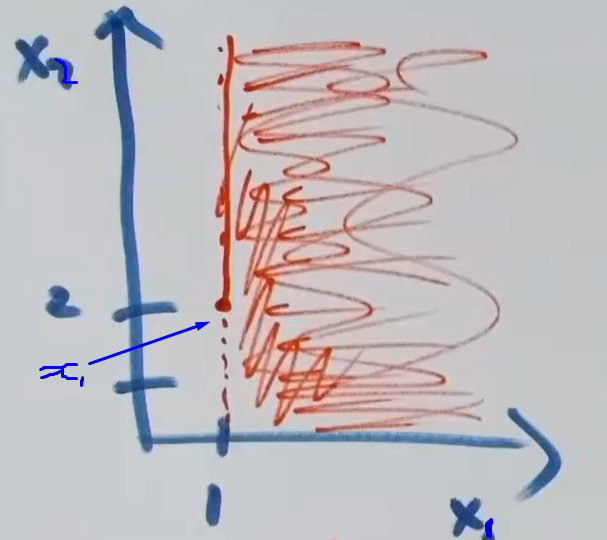
\includegraphics[width=4cm, height=3cm]{pic11}
    \end{itemize}
    \item  \underline{Defining by Strict and Indifference Preferences}: from $\succeq$ we have that:
    \begin{itemize}
      \item  \underline{A}: $\sim = \left\{(x,y) \in \mathbb{R}_{+}^{n} \times \mathbb{R}_{+}^{n}: \ x = y \right\}$ so each bundle is indifferent only to itself
      \item  \underline{B}: $\succ = \left\{(x,y) \in \mathbb{R}_{+}^{n} \times \mathbb{R}_{+}^{n}: \ x_{1} > y_{1} \ \text{or} \ (x_{1} = y_{1} \ \text{and} \ x_{2} > y_{2}) \right\}$ so a bundle is strictly preferred to another if and only if it has more of the first good or equal amounts of the first and more of the second.
    \end{itemize}
  \end{itemize}
\end{itemize}
\subsubsection{Consumer Choice Axioms}
All bundles in the subset can be compared (completeness), choices are consistent (transitivity), the consumer can choose all bundles in the subset (continuity), and more is always better (strict monotonicity). These four axioms must hold for preferences to be considered 'rational'
\begin{itemize}
  \item  \underline{Axiom 1 - Completeness}: for all $x_{1}$ and $x_{2}$ in $X$, either $x_{1} \succeq x_{2}$ or $x_{2} \succeq x_{1}$
  \item  \underline{Axion 2 - Transitivity}: for any three elements $x_{1}, x_{2}, x_{3}$ in $X$, if $x_{1} \succeq x_{2}$ and $x_{2} \succeq x_{3}$ then $x_{1} \succeq x_{3}$
  \begin{itemize}
    \item  \underline{Note}: although we require only that the consumer be capable of comparing two alternatives at a time, the assumption of transitivity requires that otther pairwise comparisons be linked together in a consistent way
    \item  \underline{Transitivity Transfers to Indifference and Strict}: suppose that preferences $\succeq$ are transitive, then:
    \begin{itemize}
      \item  \underline{1}: indifference and strict preferences are transitive
      \item  \underline{2}: for all $x, y, z \in \mathbb{R}_{+}^{n} \times \mathbb{R}_{+}^{n}$ if $x \succeq y$ and $y \succeq z$ (with one indifference), then $x \succeq z$
      \item  \underline{3}: for all $x, y, z \in \mathbb{R}_{+}^{n} \times \mathbb{R}_{+}^{n}$ if $x \succeq y$ and $y \succeq z$ (with at least one strict), then $x \succ y$
    \end{itemize}
  \end{itemize}
  \item  \underline{Axiom 3 - Continuity}: for all $x \in \mathbb{R}_{+}^{n}$, the "at least as good as set" $\succeq (x)$ and the "no better than" set $\preceq (x)$ are closed in $\mathbb{R}_{+}^{n}$
  \begin{itemize}
    \item  \underline{Conditions from Definition} preferences are continuious if $G(x) = \left\{ y \in \mathbb{R}_{+}^{n}: \ y \succeq x \right\}$ and $W(x) = \left\{ y \in \mathbb{R}_{+}^{n}: \ x \succeq y \right\}$ are both closed in $\mathbb{R}_{+}^{n}$
    \item  \underline{Theorem 1}: suppose that preferences are complete. Then, they are continuous if and only if for all $x \in \mathbb{R}_{+}^{n}$ the sets $SG(x) = \left\{ y \in \mathbb{R}_{+}^{n}: \ y \succ x \right\}$ and $SW(x) = \left\{ y \in \mathbb{R}_{+}^{n}: \ x \succ y \right\}$ are open in $\mathbb{R}_{+}^{2}$
    \begin{itemize}
      \item  \underline{Logic}: $SG(x)$ follows by definition of continuity and completeness when taking the complement of $G(x)$, $SW(x)$ follows by definition of continuity and completeness when taking the complement of $W(x)$
    \end{itemize}
  \end{itemize}
  \item  \underline{Axiom 4 - Strict Monotonicity}: for all $x_{0}, x_{1} \in \mathbb{R}_{+}^{n}$, if $x_{0} \geq x_{1}$ then $x_{0} \succeq x_{1}$ while if $x_{0} > x_{1}$ then $x_{0} \succ x_{1}$
  \begin{itemize}
    \item  \underline{Alternative Definition}: if $x$ has at least as much of each good as $y$ and strictly more of some good, then $x \succ y$
    \begin{itemize}
      \item  \underline{Note}: by completeness of preferences, the alternative definition implies the first definition
    \end{itemize}
  \end{itemize}
\end{itemize}
\subsubsection{Intermediate Value Version of Continuity}
If the preferences are continuous and complete, then for any $x, y, z \in \mathbb{R}_{+}^{n}$, if $x \succ y$ and $y \succ x$, then there is some $\alpha \in (0,1)$ such that the convex combination $\alpha x + (1- \alpha)z$ is indifferent to y. This resembles the \textit{intermediate value theorem}
\begin{itemize}
  \item  \underline{Proof}: this can be proved using completeness and continuity together with the least upper bound property (i.e. that every non-empty set of reals that is bounded above, has a least upper bound). We know that $x \succ y$ and $y \succ z$ and that the preferences are continuous. We need to show that there is some point on the line between $x$ and $z$ that is indifferent to $y$. Consider the set $A = \left\{ \alpha \in [0,1]: \ y \succ \alpha x + (1- \alpha)z \right\}$. It stands that $\alpha = 0$ is an element of $A$ since $0x + (1 - 0)z = z$ and $y \succ z$, therefore $A$ is a set of reals. It also stands that $\alpha = 1$ is not an element of $A$ since $1x + (1-1)z = x$ and $x \succ y$, therefore $A$ is bounded above by $1$ and must have a least upper bound. Call the least upper bound $\alpha^{*}$, we can show that $\alpha^{*}x + (1 - \alpha_{*})z \sim y$ using the following steps:
  \begin{itemize}
    \item  \underline{Step 1}: show that $0 < \alpha^{*} < 1$ using completness and continuity around $x$ and around $z$. For $0 < \alpha^{*}$ we have that by continuity theorem 1, since $y \succ z$, there is an open ball $B_{\varepsilon}(z)$ around $z$ such that every $z'$ in that ball that can be compared to $y$ satisfies $y \succ z'$. By completeness, all the stuff in the ball can be compared to $y$, in particular the stuff that is also on the line between $x$ and $z$. Therefore, it must be that $0 < \alpha^{*}$. For $\alpha_{*} < 1$ we have that by continuity theorem 1, since $x \succ y$, there is an open ball $B_{\varepsilon}(y)$ around $y$ such that every $y'$ in that ball that can be compared to $x$ satisfies $x \succ y$. Likewise, by completeness, it must be that $\alpha^{*} < 1$
    \item  \underline{Step 2}: show that $\alpha^{*}x + (1 - \alpha_{*})z \sim y$ using completeness and continuity. By completeness either (1) $\alpha^{*}x + (1-\alpha^{*})z \succ y$, (2) $y \succ \alpha^{*}x + (1-\alpha^{*})z$, or (3) $\alpha^{*}x + (1-\alpha^{*})z \sim y$. Options (1) and (2) cannot be the case because \begingroup\color{blue} tutorial question \endgroup. Therefore, we are left with option (3), $\alpha^{*}x + (1-\alpha^{*})z \sim y$.
  \end{itemize}
  \item  \underline{Usefulness}: this means that something on the line connecting $x$ and $z$ is indifferent to $y$
  \begin{itemize}
    \item  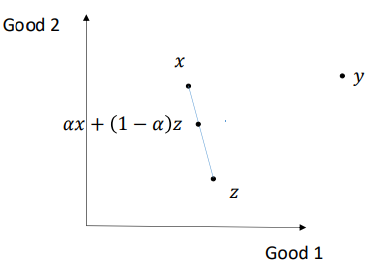
\includegraphics[width=4cm, height=3cm]{pic9}
  \end{itemize}
\end{itemize}
\subsubsection{Utility Representation}
A utility representation of preferences $\succeq$ is a real valued function $u: \mathbb{R}_{+}^{n} \rightarrow \mathbb{R}$ over the set of bundless such that for all bundles $x,y \in R_{+}$: \\ (a) if $x \succeq y$ then $u(x) \geq u(y)$ \\ (b) if $u(x) \geq u(y)$ then $x \succeq y$
\begin{itemize}
  \item  \underline{Alternative Definition} a real values function $u: \mathbb{R}_{+}^{n} \rightarrow \mathbb{R}$ is called a utility function representing the relation $\succeq$ if for all $x_{0}, x_{1} \in \mathbb{R}_{+}^{n}, u(x_{0}) \geq u(x_{1}) \Longleftrightarrow x_{0} \succeq x_{1}$
  \item  \underline{Strict Preferences}: $u: \mathbb{R}_{+}^{n} \rightarrow \mathbb{R}$ is a utility representation of preferences $\succeq$ if and only if for all bundles $x, y \in \mathbb{R}_{+}^{n}$: (a) if $x \succ y$ then $u(x) > u(y)$, (b) if $u(x) > u(y)$ then $x \succ y$
  \item  \underline{Theorem 1 - Existence of a Utility Representation}: if the binary relation $\succeq$ is complete, transitive, continuous, and strictly monotonic, then there exists a continuous real valued function, $u: \mathbb{R}_{+}^{n} \rightarrow \mathbb{R}$, which represents $\succeq$
  \begin{itemize}
    \item  \underline{Proof in Terms of 2 Goods}: \textbf{step 1} - show every point $x$ is indifferent to a point $y$ on the $45^{\circ}$ line which represents bundles with the same amount of each good, \textbf{step 2} - assign a utility $u(x)$ equal to the quantity of each good at the point on the diagonal that is indifferent to $x$, \textbf{step 3} - show that that if $x \succeq y$ then $u(x) \geq u(y)$, \textbf{step 4} - show that if $u(x) \geq u(y)$ then $x \succeq y$
    \begin{itemize}
      \item  \underline{Step 1}: if $x$ is on the $45^{\circ}$ line, we are done as by completeness $x \sim x$. Consider $x$ not on the $45^{\circ}$ line, let $\widetilde{x}$ be the bundle on the $45^{\circ}$ line where the amount of each good is the larger of $x_{1}$ and $x_{2}$ (e.g. if $x = (5,2)$ then $\widetilde{x} = (5,5)$). Since $\widetilde{x}$ has more of at least one good and at least as much of each of the others then $\widetilde{x} \succ x$ by strict monotonicity. Also, by strict monotinicity $\widetilde{x} \succ z$, where $z$ is the origin $(0,0)$. Hence, there is a point on the diagonal that is indifferent to $x$ by the \textit{intermediate value version of continuity} (i.e. $\exists \alpha, x = \alpha \widetilde{x} + (1-\alpha)z$). Note that, by strict monotonicity, there is only one bundle on the diagonal that is indifferent to $x$ referred to as $x^{d}$ where $x^{d} \sim x$
      \begin{itemize}
        \item  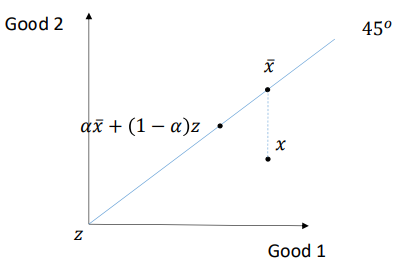
\includegraphics[width=4cm, height=3cm]{pic10}
      \end{itemize}
      \item  \underline{Step 2}: take the example where $x = (5,2)$ and the point on the diagonal that is indifferent to $x$ is $x^{d} = (2.5, 2.5)$ which yields $u(x) = 2.5$. Clearly, $u(x^{d}) = u(x)$ since $x^{d} = x$ in this case
      \item  \underline{Step 3}: suppose $x \succeq y$ and that by definition $x^{d} \sim x, y \sim y^{d}$. Therefore by transitivity we have that $x^{d} \succeq y^{d}$ and by strict monotonicity we can infer that $u(x^{d}) \geq u(y^{d})$.
      \begin{itemize}
        \item  \underline{Logic}: since $x^{d}$ and $y^{d}$ are both on the diagonal whereby $x^{d} = (a, a)$ and $y^{d} = (b,b)$ for some quantities $a$ and $b$. By strict monotonicity, combined with $x^{d} \succeq y^{d}$, we can infer that $a \geq b$. This is as, if on the contrary $b > a$, then $y^{d}$ would have more of each good than $x^{d}$. This would imply, by strict monotonicity, that $y^{d} \succ  x^{d}$. Since this would contradict the finding that $x^{d} \succeq y^{d}$, then it must be that $a \geq b$. Since $a$ represents the quantity of each good in $x^{d}$ and $b$ represents the quantity of each good in $y^{d}$, the utility function defined in step 2 will assign $u(x^{d}) = a$ and $u(y^{d}) = b$. Since $a \geq b$, we conclude that $u(x^{d}) \geq u(y^{d})$.
      \end{itemize}
      From $u(x^{d}) \geq u(y^{d})$ and $x^{d} \sim x, y \sim y^{d}$ we can infer that $u(x) \geq u(y)$. This is as by applying our utility function from step 2 we get $u(x) = u(x^{d}) \geq u(y^{d}) = u(y)$ and therefore $u(x) \geq u(y)$
      \item  \underline{Step 4}: \begingroup\color{blue} homework from priscilla notes \endgroup
    \end{itemize}
  \end{itemize}
  \item  \underline{Finite Sets}: if the set of alternatives is finite or countably infinite, then we get a utility representation with only complete and transitive preferences
  \item  \underline{Huge Spaces}: for the huge space $\mathbb{R}^{n}_{+}$, we can get a utility representation without monotonicity
  \item  \underline{Properties}: preferences represented by a utility function will always be complete and transitive, preferences represented by a continuous utility function will always be continuous
\end{itemize}
\subsubsection{Exercise 1}
Which are transitive, complete, and continuous? \begingroup\color{blue} do homework \endgroup
  \begin{itemize}
    \item  \underline{question 1}: $x \succeq y$ if and only if $x_{1}x_{2} \geq y_{1}y_{2}$
    \item  \underline{question 2}: $x \succeq y$ if and only if $(x_{1})^{2} + x_{2} \geq (y_{1})^{2} + y_{2}$
    \item  \underline{question 3}: $x \succeq y$ if and only if (a) $x_{1} > y_{1}$ or (b) $x_{1} = y_{1}$ and $x_{2} \geq y_{2}$
    \item  \underline{question 4}: $x \succeq y$ if and only if $(x_{1} - 3)^{2} + (x_{2} - 4)^{2} \geq (y_{1} - 3)^{2} + (y_{2}-4)^{2}$
  \end{itemize}


 \end{document}
